\section{Roadmap}
\label{sec:roadmap}

Every stage below except S0 is future work \evfut{}. Nothing after S0 has run, and every duration
is an indicative planning range. It is marked once, here. Gates read experiment results, never a
build: a stage that ends with new software and no result is a plan failure, not a pass.

The program is split into three phases so that money follows evidence. Phase~0 runs the cheapest
decisive test before any grant is requested. Phase~1 is a lean methods grant, released only if
Phase~0's gate reads continue. Phase~2 is released only if Phase~1's gate reads continue. An
external gate reader, not the owner, reads the deciding gates (\cref{sec:team}).
\Cref{fig:roadmap} shows the phases and gates. \Cref{tab:roadmap-stages} gives each stage's
hypothesis, build, gate rule and duration. \Cref{sec:workpackages} gives the work packages, and
\cref{sec:resources} the euros each gate releases.

\begin{figure}[tbp]
  \centering
  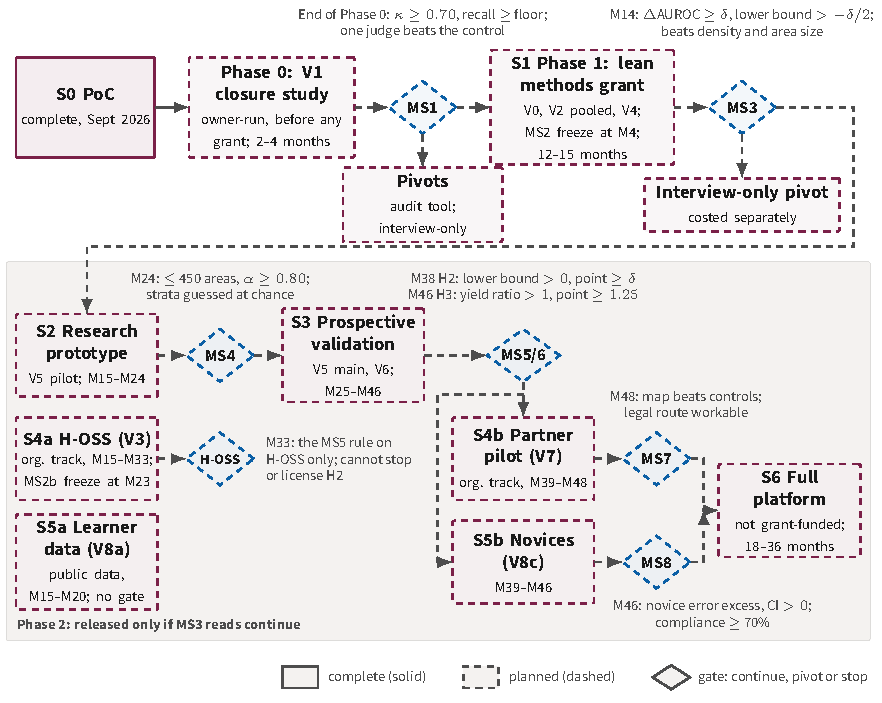
\includegraphics{figures/pdf/fig14_roadmap.pdf}
  \caption[Gated roadmap]{The roadmap in three phases, with the gate that releases each one.
  Phase~0 (owner-run, before any grant) is the closure study V1; it ends at MS1. Phase~1, a lean
  methods grant, starts only if MS1 reads continue and ends at the screening gate MS3. Phase~2
  starts only if MS3 reads continue; its prospective study decides H2 at MS5. The organizational
  track (H-OSS) runs inside Phase~2 and can neither stop nor license H2; the partner pilot waits
  for MS5.
  Every stop leads to a pivot with its own, smaller budget. Only S0 is complete.}
  \label{fig:roadmap}
\end{figure}

\begin{footnotesize}
\begin{longtable}{@{}>{\raggedright\arraybackslash}p{0.11\linewidth}>{\raggedright\arraybackslash}p{0.17\linewidth}>{\raggedright\arraybackslash}p{0.19\linewidth}>{\raggedright\arraybackslash}p{0.32\linewidth}>{\raggedright\arraybackslash}p{0.09\linewidth}@{}}
  \caption{The gated stages by phase: hypothesis tested, what gets built, the gate rule
    (continue / stop or pivot), and duration. S0 is complete; everything after it is future
    work. Months count from the start of Phase~1.}
  \label{tab:roadmap-stages}\\
  \toprule
  Stage & Hypothesis tested & What gets built & Gate: continue / stop or pivot & Duration \\
  \midrule
  \endfirsthead
  \toprule
  Stage & Hypothesis tested & What gets built & Gate: continue / stop or pivot & Duration \\
  \midrule
  \endhead
  \bottomrule
  \endfoot
  \textbf{S0 -- PoC} \evobs{} (complete) &
    H1 partly (reconstruction with provenance is feasible); H2 mechanism only &
    \code{residual/}, \code{reconstruct/}, \code{gapmap/}; three gap maps (PLC, GDPR v1, GDPR v2) &
    Closed. Engineering is complete. N2 reads inconclusive. N3 reads \enquote{pipeline complete,
      hidden-knowledge prediction not demonstrated} (\cref{sec:n2,sec:n3}) &
    Done \\
  \textbf{Phase~0 -- Closure study} (V1), owner-run, before any grant &
    L1: the absence check can be judged reliably, and retrieval finds a stating sentence where
      one exists &
    A closure codebook with anchors per lens; at least 100 double-coded units; a corpus-level
      retrieval-recall check; a judge panel scored against the fair control &
    \textbf{MS1 (closure verdict).} Continue if human $\kappa\geq0.70$, retrieval recall meets
      its floor, and one judge beats the fair control by the margin. Then write the Phase~1
      proposal with these numbers on page~1. Otherwise stop the automated absence check and take
      a pivot (\cref{sec:risks}) &
    2--4 mo \\
  \textbf{Phase~1 -- S1 Lean methods grant} (V0, V2 pooled, V4) &
    L0: trustworthy inputs. L2 (screening): the map beats the strongest baseline and adds value
      over density and area size on retrospective gold. L3: the residual is measurable &
    The area score; dated-corpus mode; the MS2 freeze at about M4 (the judge from MS1, then
      lexicons, thresholds, judge and area score hash-frozen, then gold acquired); the judge
      checked on each dated reconstruction's text &
    \textbf{MS3 (screening gate, not a verdict on H2).} Release Phase~2 only if the pooled
      $\Delta$AUROC point estimate is $\geq\delta$, its lower 90\% bound is $>-\delta/2$, and
      the map adds value over density and area size. Otherwise stop H2 funding and take the
      interview-only pivot. There is no inconclusive route &
    12--15 mo; MS3 at about M14 \\
  \textbf{Phase~2 -- S2 Research prototype} (V5 pilot) &
    Blind prospective elicitation is feasible at the powered size &
    An elicitation workbench: question service, blind-arm separation, World C records, coding
      tools, residual accounting. Track A components reused by copy, never import &
    \textbf{MS4.} Release V5's main study only if the pilot's projected number of areas fits
      the funded ceiling of 450, segmentation reaches $\alpha\geq0.80$, and stratum guessing
      stays near chance. Otherwise stop before the main study; H2 is reported as untested, and no
      underpowered V5 is run &
    M15--M24 \\
  \textbf{S3 -- Prospective validation} (V5 main, V6) &
    L4: predictions hold on fresh blind elicitation in held-out domains; this decides H2. H3:
      targeted questions yield more validated items per expert hour &
    The workbench for two held-out domains; leave-one-domain-out runs; expected information gain
      (EIG) question selection (future work N6) &
    \textbf{MS5 (H2 verdict).} Stop if the upper 90\% bound of $\Delta$AUROC is $<\delta$.
      Continue if the lower bound is $>0$ and the point estimate is $\geq\delta$. Anything else is
      reported as not supporting H2 and ends H2 funding. \textbf{MS6 (H3).} Continue if the
      yield-ratio lower bound is $>1$ and the point estimate is $\geq1.25$; any other reading
      counts against H3 &
    M25--M46 \\
  \textbf{S4 -- Organizational track} (V3, V7) &
    H-OSS: the gap map, adapted to code and commit evidence, predicts where knowledge is lost
      when developers leave. L5b: transfer to one partner &
    A World B Git adapter and code lenses, frozen at MS2b once the adapter exists; for V7, one
      tenant's ingestion, an on-prem judge stack, pseudonymization and an audit trail &
    \textbf{H-OSS gate.} The MS5 rule, on a clustered $\Delta$AUROC; it can neither stop nor
      license H2. \textbf{MS7 (V7).} Runs only after MS5 reads continue; the map beats density
      and random controls in both parts, and the legal route is workable &
    H-OSS M15--M33; V7 M39--M48 \\
  \textbf{S5 -- Education pilot} (V8a, V8c, materials) &
    L5c: confirmed residual areas carry more novice errors; teaching validated residual items
      changes a delayed outcome &
    Materials built \emph{only} from criterion-labeled, validated items (\cref{sec:platform}); a
      novice task set; manipulation-check logging &
    \textbf{MS8.} Continue if the error-excess interval lies above 0 and compliance is
      $\geq70\%$. No excess: expert residual and learner difficulty are different constructs, and
      no learner-facing feature uses the residual score. V8c starts only after MS5 reads continue &
    V8a M15--M20; V8c M39--M46 \\
  \textbf{S6 -- Full platform} (not grant-funded) &
    Commercial: residual accounting per knowledge unit is usable, legal, and worth paying for &
    A multi-tenant platform, connectors, compliance defaults in the core, a residual corpus with
    tenant isolation &
    Continue if at least two partners renew or pay and legal review is clean. MS5 not continue:
      no platform is built on the H2 claim. MS7's legal block recurs with a second partner: no
      organizational product &
    18--36 mo after S3 and S4 \\
\end{longtable}
\end{footnotesize}

\subsection{Parallel streams and where the money stops}

Phase~0 runs alone. It needs no grant, no participants and no new software, only one blind
second coder and local compute. Phase~1 runs its work in one line: build the area score and dated-corpus mode,
freeze at MS2, reconstruct, check the judge on the new text, then acquire gold and read MS3. Nothing in Phase~1 builds the
workbench, the Git adapter or any Phase~2 component, so no Phase~2 spending runs ahead of MS3.

Phase~2 has three streams. The prospective stream (S2, S3) waits for MS3, and V5's main study
waits for MS4. The organizational track (S4) starts with Phase~2, freezes its code lenses at MS2b
and reads H-OSS at its own gate. H-OSS cannot kill or license H2, and H2's gates do not read V3.
The partner pilot (V7) starts only after MS5 reads continue. The education stream runs V8a on public data early and V8c only after MS5. Validation
Track A runs on its own registered preconditions at any time; no gate here schedules or blocks it
(\cref{sec:validation}).

\begin{keyquestionbox}
  \textbf{Where the money stops.} Each phase is released by one gate, read by the external gate
  reader against the pre-registration.
  \begin{itemize}[noitemsep]
    \item \textbf{MS1 stops:} no grant is requested for the gap map. The ledger continues as a
      documentation-audit tool, or the interview-only pivot is proposed on its own budget.
    \item \textbf{MS3 does not release Phase~2:} H2 funding ends. The interview-only pivot tests
      targeted interviewing guided by expected information gain, without any reconstruction
      prior, on its own smaller budget (\cref{sec:resources}).
    \item \textbf{MS5 does not read continue:} H2 is reported as not supported, and no money is
      released for V6, V7, V8c or a platform built on the H2 claim. The interview-only pivot
      remains open on its own budget.
  \end{itemize}
  MS3 is a screening gate: it decides whether Phase~2 money is worth releasing. Only MS5 decides
  H2 as defined. No later stage can undo what either gate decides.
\end{keyquestionbox}
